%%%
\subsection{DVMS}\label{ssec:dvms}

%\subsubsection{Overview.}
DVMS~\cite{quesnel:ispa2013,quesnel:cpe2012} (Distributed Virtual Machine Scheduler) is a
framework that schedules VMs cooperatively and dynamically in large scale distributed
systems. It is deployed as a set of agents that are organized following a ring topology
and that cooperate with one another to guarantee that VM demands are satisfied during
their executions. Concretely, when a node cannot guarantee the QoS for its hosted VMs or
when it is under-utilized, it starts an iterative scheduling procedure~(ISP) by querying
its first neighbor to find a better placement; it thus becomes the initiator of the ISP.
If the request cannot be satisfied by the neighbor, it is forwarded to the following free
one until the ISP succeeds. When a viable mapping has been found, the leader (\ie the last
peer that has taken part to the ISP) reconfigures the system by performing adequate VM
migrations. Such an approach allows each ISP to send requests only to a minimal number of
nodes and even though an ISP can reserve all nodes if the corresponding problem is
particularly hard to solve (guaranteeing thus that a solution will always be found if it
it exits), experiments have shown that in most cases ISPs involve only few
nodes. Moreover, the DVMS proposal allows several ISPs to occur independently at the same
moment throughout the infrastructure; in other words, scheduling is performed on
partitions of the system that are created dynamically, which significantly improves the
reactivity of the system. To prevent conflicts that could occur if several ISPs performed
concurrent operations on the same PMs or VMs, it should be noted that PMs are reserved for
exclusive use by a single ISP.

An example involving three partitions is shown in Figure~\ref{fig:isp}; in particular, we
can see the growth of partition~1 between two steps. Explaining in details the notion of
``first out'' is beyond the scope of this article but readers can consider that the
``first out'' relation enables to handle communications efficiently, as each node involved
in a partition can forward a request directly to the first node outside its
partition~\cite{quesnel:cpe2012}.

\begin{figure}[h!]
  \centering
  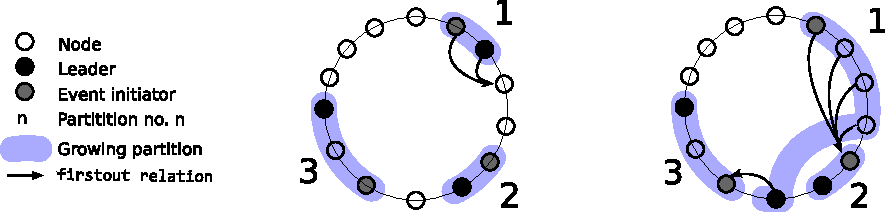
\includegraphics[width=0.9\linewidth]{Figures/resourceAcquisition-standard.pdf}
  \caption{Solving three problems simultaneously and independently with DVMS.}%
\small{The ring has been matched on top of three distinct clusters.}
  \label{fig:isp}%
\end{figure}

In addition to formally prove the correctness of DVMS, the first version of the prototype
has been validated at large scale (up to 80k VMs and 8k nodes by means of simulations and
up to 4.7k VMs and 470 nodes by means of experiments over the Grid'5000
testbed~\cite{quesnel:ispa2013}).

As discussed earlier, one limitation of this approach is related to its ring topology that
prevents to take into account the actual network topology.
%\subsubsection{Limitations of The Ring}
%
%Even though  DVMS can be deployed across several sites, it performs better on a
%cluster.
%
%The reason is simple.
%
%The ring is built without taking account of the network  topology; 
In other words, if the ISP strategy enables to limit the size of one partition to a
minimal number of nodes, these nodes are selected without considering the network
conditions at the time the ISP starts; leading to inefficient situations where VM
migrations occur between two nodes that are far from each other, which lasts longer than a
migration between two close nodes. Obviously the ring can be built in order to limit the
distance between peers globally (\ie peers of the same region/area would be grouped
together as illustrated in Figure \ref{fig:isp}). However, in such a case, at least two
nodes of each group are directly connected to two far nodes.
%
Note that an approach such as the one proposed in~\cite{superchord} that consists in
deploying one ring per site and interconnect these rings through a \emph{super-ring}
interconnecting few representatives of each local rings, would not solve many
problems. Besides problems inherent to hierarchical and structured overlay networks, this
solution would not provide a good answer to locality: when going out of the local ring, it
would still not be possible to find the next closest ring.
%
%To sum up, the DVMS proposal lacks of a topology that can consider locality
%properties of a multi-sites infrastructure. 

% Autres limitations :
% -absence de tolerance aux pannes
% -peu d'evenements geres (surcharge d'un noeud)
% -ne prend pas en compte les liens entre VMS

\subsection{Overlay Networks and Locality}

As illustrated in the previous paragraph, one of the primary downsides of overlay networks
lies in that they break the physical topology by connecting nodes that have no physical
proximity.
%
Besides hierarchical attempts in building locality aware overlay
networks~\cite{superchord,ECAN,XuMK03}, we can first mention the locality
improvement mechanisms of the Pastry structured overlay
network~\cite{pastry}. In order to reduce the latency of the routing process,
each node is given the opportunity to choose the closest nodes to fill its
routing table. Learning the existence of new nodes relies on a periodic exchange
of parts of routing tables.

Similar mechanisms have been adopted within unstructured overlay networks to make their
logical connections reflect the physical proximity of nodes, each node discovering its
closest nodes through gossiping. Note that the proximity between two nodes can be
estimated through any transitive metric, in particular the latency between the
nodes~\cite{tman}.

These approaches need to constantly maintain the knowledge of close nodes in order to
provide the \emph{best} node possible at the cost of periodic communications (uncorrelated
to the actual amount of requests to be processed by the overlay).

The overlay we propose in this paper differs in that it adopts a lazy approach consisting
in searching close nodes upon receipt of requests. This way, the quality of the response
is proportional to the frequency of requests.

Our protocol relies on the Vivaldi protocol~\cite{dabek:2001:sigcomm04} to detect close
nodes. Vivaldi places nodes in a multi-dimensional space. Each node is given coordinates
inside this space reflecting its physical location. The protocols is based on simple
message exchanges. Initially, each node is given a random position in the space and
chooses (possibly arbitrarily) a small subset of nodes, composing its \emph{view}. Then,
each node, starts estimating the round trip time between itself and another node chosen
randomly in its view, and adapts its distance with this node in the space accordingly,
coming closer to it or moving away from it. This step can be repeated by the nodes
independently (with another node in their view), to improve the acuracy of the
positioning. A globally accurate positioning of nodes can be obtained very quickly (in a
small number of steps) if nodes have a few long-distance nodes in their view and if the
network is not excessively dynamic. These long distance links can be easily maintained.

Recall that Vivaldi does not allow to directly know the nodes which are close in the
network, but to recognize them through their coordinates. Our overlay relies on the
examination of Vivaldi coordinates of nodes discovered during the processing of requests
sent to it.






